\documentclass{amsart}

\usepackage{graphicx}
\usepackage{pdfpages}

\title{CSCI 6907 Project Proposal\\
Lights Out Management}
\author{James Lee\\
\texttt{jameslee@gwu.edu}}
\date{\today}

\begin{document}
\maketitle

\section{Project Abstract}
I am a system administrator who manages hundreds of Unix systems.  One of the essential tools to ensure I don't have to visit the datacenter every time I want to work on a system is called ``lights out management'' (LOM).  It's a little device built into high-end servers that allows me to log in over the network, power the system on and off, and access the operating system's console, when more traditional methods such as SSH fail.

I run my personal file and web server at home on a Sun Ultra 24.  It's a low-end, commodity X86 system with no built-in LOM.  I've rendered it inaccessible many times while performing upgrades or configuration changes remotely.  I could have benefitted from a LOM in my home server, so I am proposing to build one.

When complete, my LOM must be able to allow me to connect to it over the network with telnet, power the system on and off, and access the system's serial console for every state the system is in (BIOS, bootloader, kernel boot, console login shell) all without modifying the server's hardware.

\section{Strategy}
The device will be built on top of the Arduino Prototyping Platform.  I chose the Arduino mostly because I already own one (an Arduino Uno) and I want to keep costs low.  This device is something I'll actually use, so I don't want to borrow any components.  The Arduino is also attractive because of the availability of ``shields'' that extend its functionality by plugging new components into the board without soldering.  An ethernet sheild and accompanying library are available for basic TCP/IP networking, and I intend to make use of them.  I also like that the Arduino can be powered by USB.  The Sun Ultra 24 has an internal USB port that always supplies power, even when the system is off.

Beyond that, I will need to find a way to add an RS-232 serial port to the Arduino.  The Arduino's ATmega328 microcontroller contains one UART for serial communication, but it is tied to the USB port, which I will need for programming and debugging.  A software serial library is available for the Arduino for bit-banging serial communication over any GPIO ports, but that could impact the device's performance and interactivity due to the precise timing required for high-speed serial communication.  And besides, that's too easy.  So I will add a second hardware UART to the Arduino to connect to the system's serial console.

Traditional UARTs, such as the 16550, require more pins than the Arduino has, so I need to choose a UART with a more efficient bus technology, such as SPI which only requires four pins.  After careful consideration, I have chosen to implement the Maxim MAX3110E in my project.  It's a combination of an SPI compatible UART and RS-232 transceiver.  It's available in a DIP package, so I could effectively run wires from my Arduino to the MAX3110E and from there to the serial port headers on the system's motherboard.  I intend to take advantage of the interrupt raised by the chip to know when to read data from its eight word FIFO queue, rather than polling it.

I will also need to develop the circuits necessary for controlling the system's power.  My goal will be to be able to turn the system on and off, and reset it.  To do this, it will be helpful for my device to know the current power state of the system.  I plan to detect the system's state from its power LED.  I will redirect the LED power line from the motherboard to a circuit connected to my Arduino to detect its state, and connect the power LED to the circuit such that it remains functional.  I've already proved the concept using a couple of transistors:

\begin{center}
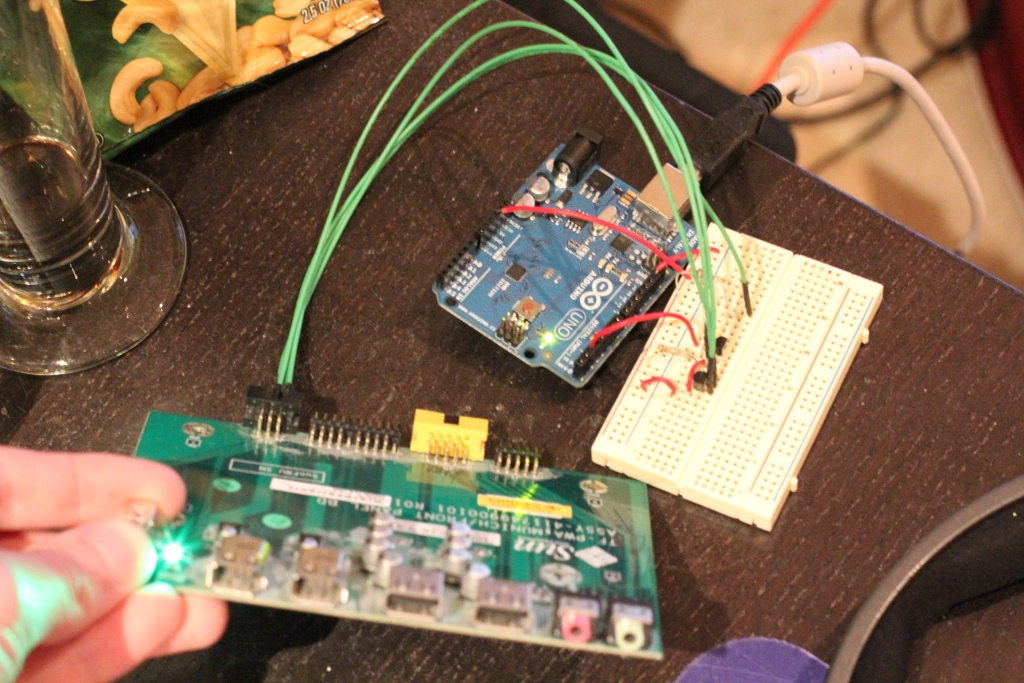
\includegraphics[width=.9\textwidth]{pled.jpg}
\end{center}

A pin is also available on the system's motherboard that will help me control power.  From my observation, it is pulled high to 3.3 V.  When it drops low (i.e. gets pulled to ground), the system turns on.  If it's pulled low for five seconds, the system turns off.  That's how the power button on the front of the computer works.  It's a simple button connected between the power pin and ground.  Again, with a transistor or two and I should be able to control that from my Arduino without affecting the operation of the physical power button.

\begin{center}
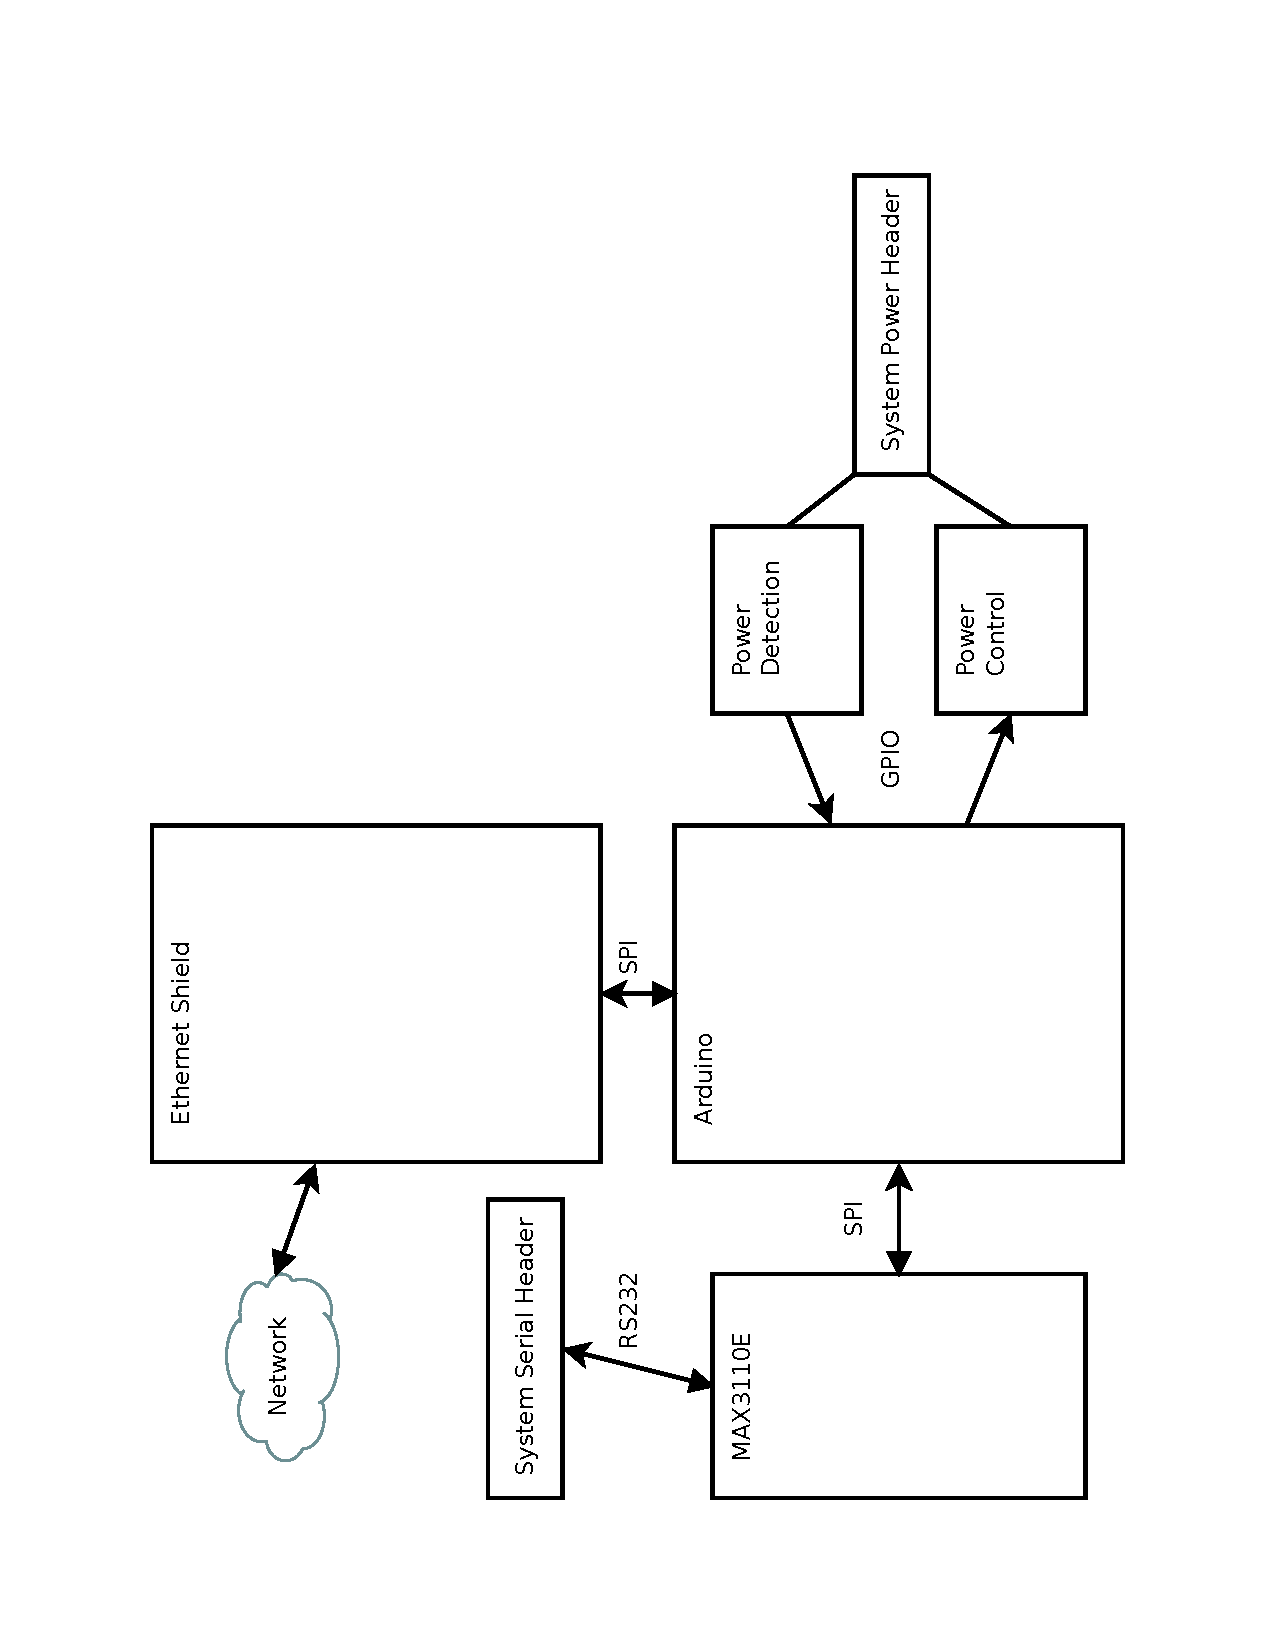
\includegraphics[height=\textwidth,angle=270]{hw-block.pdf}
\end{center}

On top of the hardware, I will develop software that pulls all of the pieces together into a simple command-line interface.  I will use the Arduino ethernet library to get an IP address from DHCP, accept connections over TCP port 23, and send and receive data from the stream.  I will also write a driver that controls the MAX3110E over SPI.  Ideally it will extend the Arduino streams library to present an interface consistent with the other Arduino I/O libraries.  Then I will write any code necessary to transmit data between the telnet and serial interfaces.  Time permitting, I will make it possible to configure the LOM device, including settings such as IP address and serial port baud rate, over the telnet interface, saving the settings in the Arduino's EEPROM.  The interface should look something like:

\begin{verbatim}
jlee@client% telnet arduino
> help
Available commands:

  status
  poweron
  poweroff
  reset
  console
  exit

> status
System is off.
> poweron
> status
System is on.
> console
Press #. to exit console.

system login: jlee
password: 
jlee@system % exit
#.
> exit
Connection closed by foreign host.
jlee@client %
\end{verbatim}

\section{Unknowns}
The biggest unknown for me is whether I'll be able to implement the MAX3110E chip.  I've never worked with SPI before so it may be a challenge to learn.  Complicating matters is that the Arduino ethernet shield also operates on the same SPI bus.  Some forums discussions indicate the shield's ethernet module, the Wiznet W5100, has a poor SPI implementation that pollutes the MISO line even it's not selected.  Others seem to have gotten around the issue by completely disabling SPI on the W5100 while it's not in use.  This may require modification to the ethernet shield itself, and will almost certainly require modification to the ethernet library.  It will be the first issue I have to resolve when I receive the parts.

I also wonder whether I will be able to acheive the oscillator accuracy required for driving the MAX3110E from a breadboard.  The datasheet warns about keeping traces between the MAX3110E and the crystal oscillator short due to parasitic capacitance, something I can't really control in a breadboard.  It says the chip will operate with up to a 1\% error in the oscillator.

Another fear is the 32 KB program size limitation on the Arduino.  Simple input-output programs can take 6 to 8 KB, and basic client-server networked programs using the ethernet library take about 16 KB.  I will have to budget the code space very carefully.  I may have to get creative towards the end to get everything to fit.  I know I can jettison the DHCP piece to save ~3 KB if I have to.

A lesser fear is that I will not be able to drive the Arduino, the ethernet shield, and the MAX3110E from the current supplied by the USB port.  If not, I can connect it to a wall wart.

\section{Implementation Plan}
\begin{tabular}{lp{4in}}
Week Of & Milestone\\
\hline
Feb 12 & Order parts\\
Feb 19 & Receive parts, confirm serial console access with laptop, develop circuits for power control.\\
Feb 26 & Begin work on MAX3110E driver.\\
Mar 4 & Be able to talk back and forth between serial ports on the Arduino.\\
Mar 11 & Build small proof of concept app using the ethernet shield and library; test interoperability with MAX3110E on shared SPI bus.\\
Mar 18 & Solidify network and serial layers; develop power control library; bring pieces together into command-line user-interface.\\
Mar 25 & Project completed.\\
\end{tabular}

\section{Resources}
\begin{itemize}
\item Sun Ultra 24
\item Arduino Uno
\item Arduino Ethernet Shield
\item Maxim MAX3110E
\item 3.6864 MHz Crystal Oscillator
\item 2 33 pF Capacitors
\item General Purpose NPN Transistors
\item Breadboard and Jumper Wires (M-M and M-F)
\end{itemize}

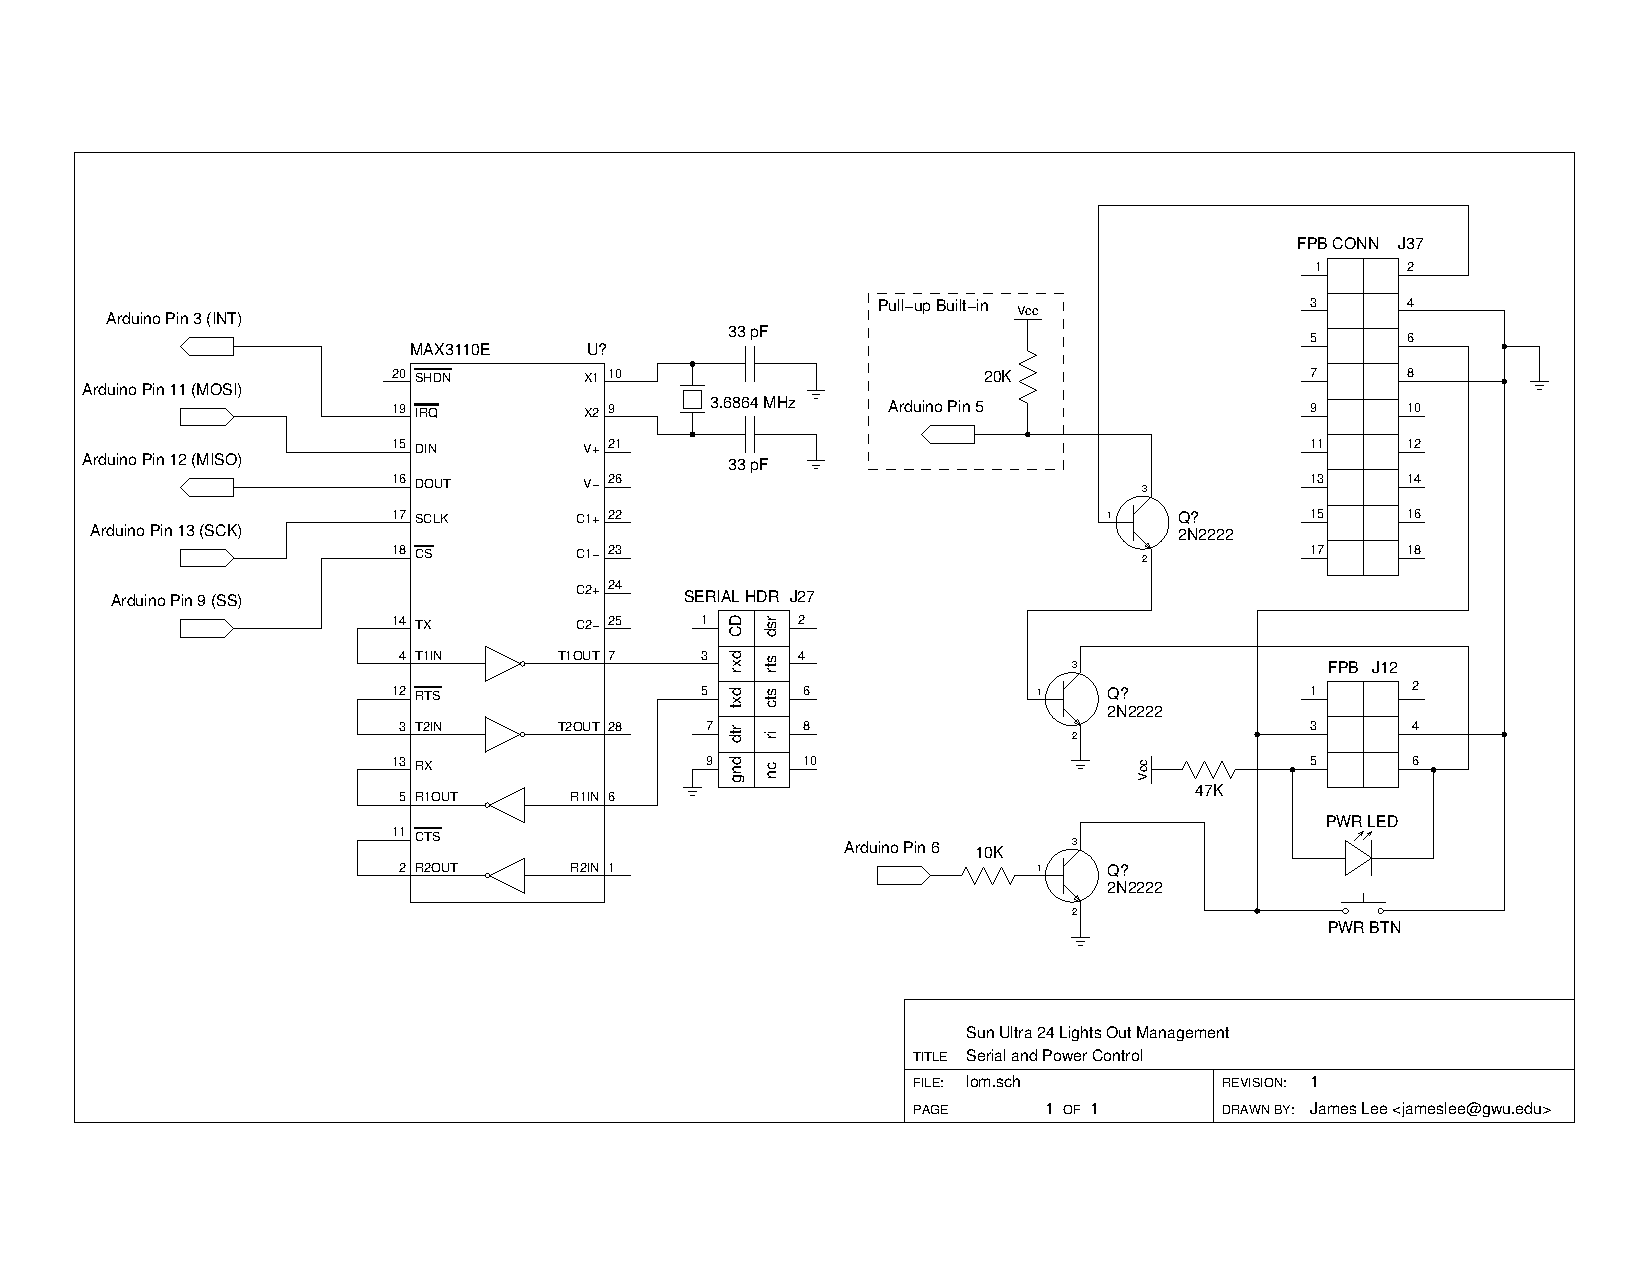
\includepdf[landscape]{schematic.pdf}
\end{document}
